\documentclass[11pt,border=4pt]{standalone}
\usepackage{amsmath,amssymb,bm,mathtools}
\usepackage[fontset=fandol]{ctex}
\usepackage{tikz}
\usetikzlibrary{arrows.meta,calc,patterns,angles,quotes,decorations.markings,decorations.pathmorphing}
\newcommand{\dd}{\mathop{}\!\mathrm d}
\newcommand{\e}{\mathrm e}
\tikzset{axis/.style={->,>=Stealth,line width=.45pt},world/.style={line width=.8pt},flow/.style={->,>=Stealth,line width=.7pt},ray/.style={->,>=Stealth,line width=.7pt},guide/.style={dashed,line width=.35pt},aux/.style={dashed,line width=.35pt},dim/.style={<->,>=Stealth,line width=.35pt},every node/.style={font=\small},force/.style={->,>=Stealth,very thick},gas/.style={fill=blue!7}}
\begin{document}
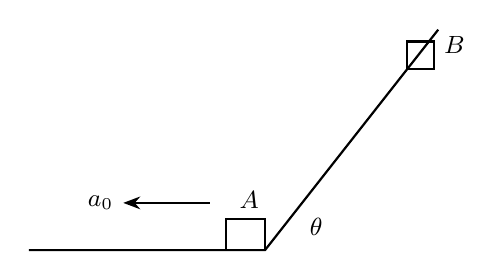
\begin{tikzpicture}\draw[world](-3,0)--(0,0)--(2.2,2.8);\draw[world](-.5,0)rectangle(0,.4);\draw[world](1.8,2.3)rectangle(2.15,2.65);\node[above]at(-.2,.4){$A$};\node[right]at(2.15,2.6){$B$};\draw[flow](-.7,.6)--(-1.8,.6)node[left]{$a_0$};\node at(.65,.3){$\theta$};\end{tikzpicture}
\end{document}
